\section{Method}
\label{sec:method}

Our approach assumes that we have been given as input: (1) a user-selected visualization which the user wants to partition into a small multiple display, (2) a quality measure defined on this visualization type that captures patterns of interest to the user, and (3) the data set underlying the visualization which includes additional variables not mapped to visual variables that are potential partitioning variables in a small multiple display. The output of our method is a scoring of the small multiple displays produced by each partitioning variable.

\subsection{Goodness-of-Split Criteria}
We would like our approach to select small multiple displays that have the following four properties:
\begin{itemize}
\item \emph{Visually rich}: We want small multiple displays that convey rich visual patterns, as captured by the quality metric provided by the analyst. In contrast to statistical methods, such as ANOVA, which are based on relatively simple summary metrics with closed-form distributions under some assumptions, most visualization quality metrics involve complicated processing and do not follow a known distribution.

\item \emph{Informative}: The purpose of a small multiple display is to help explain patterns in the input visualization. We want our method to pick partitioning variables that are likely to be informative. Partitions that randomly split the data are not useful.

\item \emph{Well-supported}: For some data sets, particularly those with outliers or with a small number of data points, high quality scores can occur by chance. We would like to detect and downweight spurious patterns in such displays.

\item \emph{Parsimonious}: A small multiple display with many partitions can be very difficult to read and understand. All things being equal, we want to favor splitting into as few plots as possible, while still providing an informative display.
\end{itemize}

\subsection{Algorithm}

\begin{figure}
 \centering 
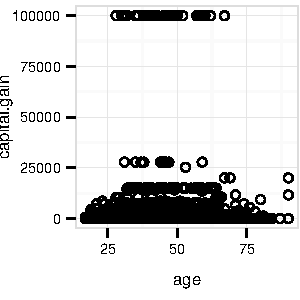
\includegraphics[width=1.5in]{images/age-capital_gain.pdf}
  \caption{Original interesting bivariate relationship}
 \label{fig:method_original}
\end{figure}

%Given a user-selected set of response variables, we want to automatically find a good Split respecting the criteria outlined above. This process of selecting a good Split, adding a conditioning variable to explain the visual structure in a set of data observations when we have many potential such variables, is akin to the model selection process. We evaluate the ``model" a Split determines based not only on the quality of the interesting patterns in partitions, but also, on the simplicity or size of the collection of partitions. Model selection is commonly employed in statistics and data mining to pick a statistical model that fits a sample of data, such as curve fitting or clustering. However, applying such a methodology with cognostics or visual pattern measures studied in the information visualization community has not been explored. We describe an algorithm to apply cognostics to do model selection where a model is determined as the addition of an explanatory variable to a selected set of response variables. 


Our approach is based on a permutation test, which is a non-parametric statistical significance test where the distribution of a test statistic under the null hypothesis is determined by computing the test statistic on rearrangements of the observed data points. Here, we find the statistical significance of a particular small multiple display using a cognostic as the test statistic. This allows us to evaluate small multiples for patterns not due to chance, so we can automatically find a good small multiples.

To understand how this algorithm works, consider the example in Figure~\ref{fig:method_original}. Blah blah about the dataset...

Central to our approach is the use of a cognostic that tracks the visually interesting pattern we seek to distinguish in a Split. The cognostic is an independent, substitutable piece of the approach and its choice is based on the user's task and interest. For this example, we use the Clumpy scagnostic measure~\cite{Wilkinson2005} as our cognostic.

Let the partitioning variable $d_p$ create $k$ partitions with sizes $\left\{ {s_1, s_2,...,s_k}\right\}$. We compute the cognostic on each of these $k$ partitions to get a set of interestingness measures $\left\{ {c_1, c_2,...,c_k}\right\}$. Figure~\ref{fig:method_actual} shows the small multiple resulting from using the "Relationship" variable to partition the original view. The partitions, going from the top of the bottom, have sizes $\left\{ {6523, 4278, 525, 2513,1679, 763}\right\}$  and Clumpy measures $\left\{ {0.033, 0.038, 0.086, 0.019, 0.042, 0.049}\right\}$.

\begin{figure*}
 \centering 
	 \begin{subfigure}{1.25in}
 	\centering 
  		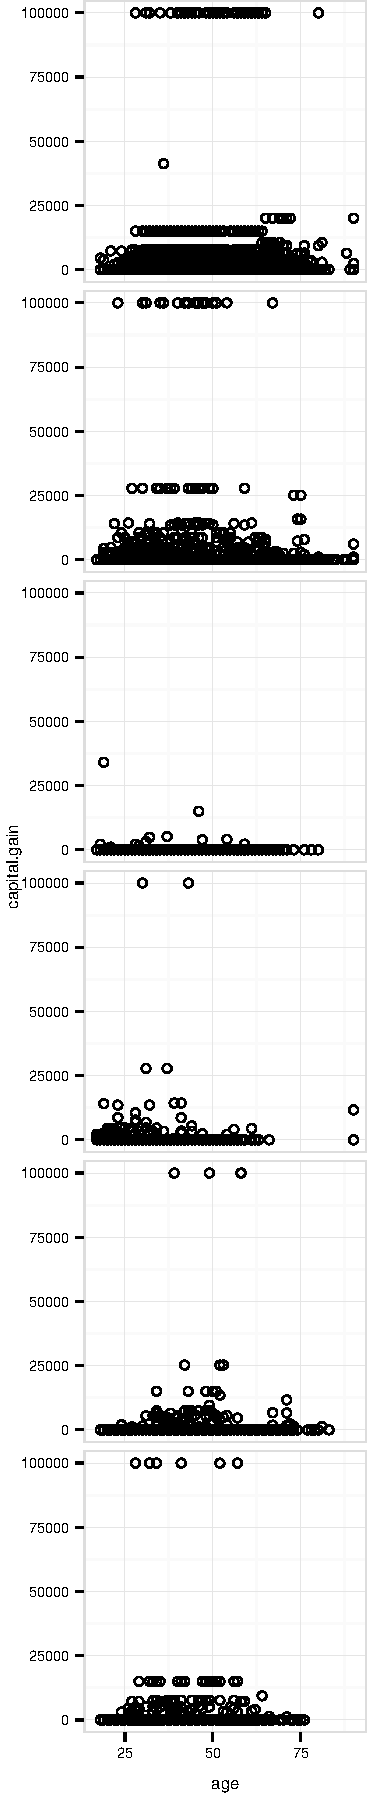
\includegraphics[width=1.25in]{images/relationship.pdf}
		\caption{}
		 \label{fig:method_actual}
	 \end{subfigure}
	 \begin{subfigure}{1.25in}
 	\centering 
 		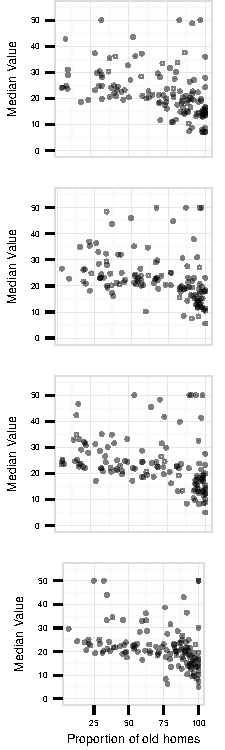
\includegraphics[width=1.25in]{images/randCluster.pdf}
		 \label{fig:method_random}
 		\caption{}
	 \end{subfigure}
	 \begin{subfigure}{2in}
 	\centering 
 		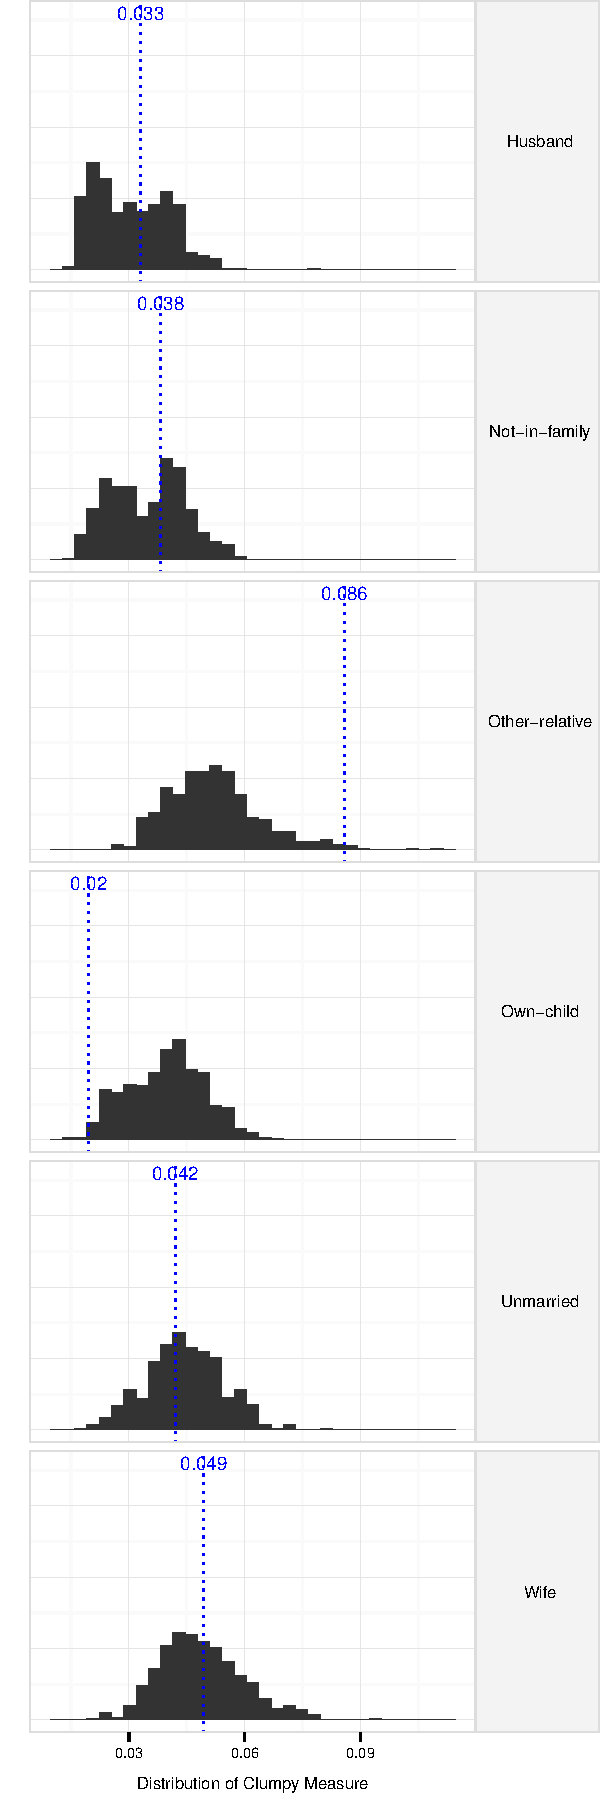
\includegraphics[width=2in]{images/hist-relationship.pdf}
		\caption{}
		 \label{fig:method_dist}
	 \end{subfigure}
   \caption{Illustration of our method of evaluating small multiple displays. (a) Partitions determined by the Relationship variable. (b)Randomly permuted partitions of data. (c) Distribution of Clumpy measures for randomly permuted partitions. The overlaid blue lines are the corresponding Clumpy measures of the partitions determined by Relationship in (a).}
\end{figure*}

Then, we generate a random permutation of the original data into $k$ partitions of the same sizes $\left\{ {s_1, s_2,...,s_k}\right\}$ as seen in Figure~\ref{fig:method_random}. We use permutation sampling as we assume our dataset is representative of the population and do not need to compensate, via bootstrapping, for the assumption that it represents a sample from a larger, unexamined population. (NEED MORE HERE). We compute the Clumpy measure on each of these $k$ random partitions. Then we generate $r$ such randomly permuted partitions and corresponding sets of measures to create $k$ distributions of cognostics as seen in Figure~\ref{fig:method_dist}. 

The generated cognostic distributions function as reference "null distributions" and we apply a non-parametric significance test to determine how significant the difference is between the partitions determined by a particular variable and random partitions. The z-score from Chebyshev's inequality is as follows:
$$\sum_{i=1}^n \frac{(x_i-\mu_i)^2}{\sigma_i^2}$$
where $x_i$ is the score of the i-th partition and $\mu_i$ and $\sigma_i$ are the mean and standard deviation of the cognostic measures for the i-th partition for the randomly-generated partitions. We use the z-scores to ranking partitioning variables and the Relationship variable produces the highest ranked small multiple at $9.995$ given the original view.

\subsection{Handling Continuous Partitioners}
Determining discrete splits for a categorical variable is trivial as the observations are naturally partitioned into subsets for each discrete choice the variable offers. For continuous variables, discrete partitions can be created through a binning technique. There are various binning techniques that split a continuous range into disjoint intervals~\cite{Freedman1981,Scott2009} employed in histograms. An alternative binning strategy is one with overlapping bins of roughly equal count called shingles~\cite{Becker1996 ?Cleveland book first??}. The overlap of the intervals increases the resolution with which we can study conditional independence in the same way that moving averages increase the resolution of local behavior at each time point. 
%Figure~\ref{fig:shingles} shows such �moving snapshots� of the data across the range of the partitioning variable.

\subsection{Multiple Partitioners}
Small multiples or trellis plots facet a single view into multiple views, each displaying subsets of data conditioned on the variables defining the small multiple. These conditioning or partitioning variables are combined using cross and nest operators~\cite{Wilkinson2005GG,Stolte2002} to define the layout of the small multiple. Our algorithm could be used to pick variables to partition on in the transition from a large single view~\cite{van2013} to informative small multiples.


